\documentclass[english,14pt]{beamer}
\usetheme{EastLansing}
\usecolortheme{spruce}

\usepackage{xcolor}
\usepackage{listings}
\usepackage{courier}
\usepackage{graphicx}
\usepackage{amsmath}
\usepackage{algorithm2e}
\usepackage{multicol}
\usepackage{hyperref}
\usepackage{textcomp}

% http://mirrors.ibiblio.org/CTAN/macros/latex/contrib/datetime2/datetime2.pdf
\usepackage{babel}
\usepackage[useregional]{datetime2}

% https://tex.stackexchange.com/questions/42619/x-mark-to-match-checkmark
\usepackage{pifont}% http://ctan.org/pkg/pifont

%% https://stackoverflow.com/questions/1435837/how-to-remove-footers-of-latex-beamer-templates
%%gets rid of bottom navigation bars
%\setbeamertemplate{footline}[page number]
%
%gets rid of navigation symbols
\setbeamertemplate{navigation symbols}{}


\usefonttheme[onlymath]{serif}

\definecolor{mGreen}{rgb}{0,0.6,0}
\definecolor{mGray}{rgb}{0.5,0.5,0.5}
\definecolor{mPurple}{rgb}{0.8,0,0.82}
\definecolor{backgroundColour}{rgb}{0.95,0.95,0.92}
\definecolor{lightBlue}{rgb}{0.1, 0.1, 0.8}
\definecolor{darkGreen}{rgb}{0, 0.39, 0}

\newcommand\red[1]{{\color{red} #1}}
\newcommand\green[1]{{\color{green} #1}}
\newcommand\blue[1]{{\color{blue} #1}}
\newcommand\darkGreen[1]{{\color{darkGreen} #1}}

\newcommand{\cmark}{\ding{51}}%
\newcommand{\xmark}{\ding{55}}%

\lstdefinestyle{CStyle}{
    backgroundcolor=\color{backgroundColour},   
    commentstyle=\color{mGreen},
    keywordstyle=\color{magenta},
    numberstyle=\tiny\color{mGray},
    stringstyle=\color{mPurple},
    basicstyle=\footnotesize,
    breakatwhitespace=false,         
    breaklines=true,                 
    captionpos=b,                    
    keepspaces=true,                 
    numbers=left,                    
    numbersep=5pt,                  
    showspaces=false,                
    showstringspaces=false,
    showtabs=false,                  
    tabsize=2,
    language=Python
}

\lstdefinestyle{pseudo}{
        basicstyle=\ttfamily\footnotesize,
        keywordstyle=\color{lightBlue},
        morekeywords={BEGIN,END,IF,ELSE,ENDIF,ELSEIF,PRINT,WHILE,RETURN,ENDWHILE,DO,FOR,TO,IN,ENDFOR,BREAK,INPUT,CONDITIONS},
        morecomment=[l]{//},
        commentstyle=\color{mGreen}
}

\lstset{basicstyle=\footnotesize\ttfamily,breaklines=true}
\lstset{framextopmargin=50pt,tabsize=2}

\title{ENGG1003 - Thursday Week 9}
\subtitle{Random numbers from normal distributions \\
---aka random numbers from Gaussian distributions}
\author{Steve Weller}
\institute{University of Newcastle}
%\date{\today}
\date{6 May 2021}

% following is a bit of a hack, but forces page numbers (technically: frame numbers) to run 1,2,3,... 
% with titlepage counting as frame 1

\addtocounter{framenumber}{1}
\titlepage

\begin{document}

\begin{flushleft}
{\scriptsize Last compiled:~\DTMnow}
\vspace*{-5mm}
\end{flushleft}
\framebreak

%==============================================================

\begin{frame}[fragile]

\frametitle{Lecture overview}
\begin{enumerate}
	\item[]
	
	\item normal distribution
	\begin{itemize}
		\item also known as \emph{Gaussian distribution} or ``bell curve''
%		\item today: ``standard'' normal ie: mean $\mu = 0$ and $\sigma = 1$ %zero and std 1, 
		\item today: draw random samples from ``standard'' normal distribution
%		\item histogram
	\end{itemize}
	
	\item[]
	
	\item compute probabilities using normal distribution
	\begin{itemize}
		\item uses numerical integration
	\end{itemize}
	
%	\item[]
%	
%	\item normal distribution (aka Gaussian)
%	\begin{itemize}
%		\item pdf, meaning of $\mu$ and $\sigma$
%		\item generate using Python
%		\item area (needs integration) and probability
%	\end{itemize}
	
%	\item[]
%	
%	\item engineering application
	
\end{enumerate}

\end{frame}

%==============================================================

\begin{frame}[fragile]

\frametitle{$1)$ Normal distribution}

\begin{itemize}
	\item intoduced \emph{uniformly} distributed random numbers in week 4
	
	\item[]
	
	\item today: introduce ``standard'' normal distribution
 	\begin{itemize}
		\item extend next week to general form
		\item also known as random numbers from \emph{Gaussian distribution}
		\item occur \emph{very} widely in all branches of Engineering
	\end{itemize}

	\item[]
	
	\item two goals today using standard normal distribution:
	\begin{enumerate}
		\item use Python to draw random samples
		\item use Python to compute probability of random number falling in specified range
	\end{enumerate}

\end{itemize}

\end{frame}

%==============================================================

\begin{frame}[fragile]

\frametitle{Standard normal distribution}

\begin{itemize}
	\item generate $100,000$ random numbers using \texttt{normal()} function in numpy's random library
	\begin{itemize}
		\item standard normal: first two parameters in call to \texttt{normal()} are $0.0$ and $1.0$
	\end{itemize}
\end{itemize}

{\small
	\texttt{x = np.random.normal(\red{0.0}, \blue{1.0}, size=100000)}
}

\vspace*{5mm}

\begin{itemize}
	\item use \texttt{hist()} function in matplotlib library to generate histograms of observed data
	\begin{itemize}
		\item $10$ bins
		\item $100$ bins
	\end{itemize}
\end{itemize}


\end{frame}

%==============================================================

\begin{frame}[fragile]

\frametitle{Python code: generate histograms}

\texttt{histdemo.py}
\begin{lstlisting}[style=CStyle,basicstyle=\scriptsize]
# histdemo
import numpy as np
import matplotlib.pyplot as plt

np.random.seed(1)
d = np.random.normal(0.0, 1.0, size=100000)

x = np.linspace(-5,5,num=1000)
f = 1/(np.sqrt(2 * np.pi)) * np.exp(-x**2 / 2)

plt.hist(d, 100, density=True)
plt.plot(x, f, color='r', linewidth=3)
#plt.hist(d, 100)

#plt.plot(d, 'o')
plt.show()
\end{lstlisting}

\end{frame}

%==============================================================

\begin{frame}[fragile]

\frametitle{Histogram: 10 bins}

\begin{figure}[ht]
	\centering
	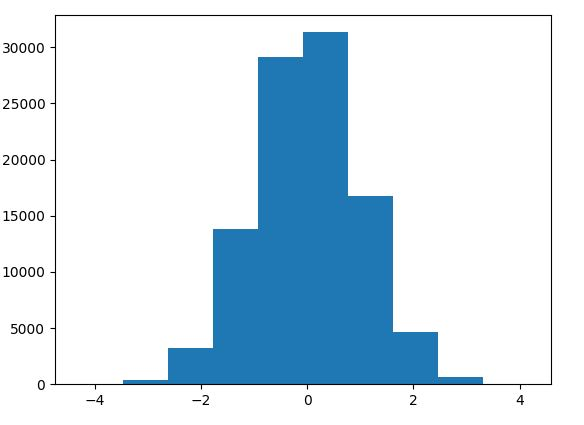
\includegraphics[width=0.7\textwidth]{figures/hist10BinsExample}
\end{figure}

\vspace*{-5mm}

\begin{itemize}
	\item height of each rectangle refects number of samples in each ``bin''
\end{itemize}

\end{frame}

%==============================================================

\begin{frame}[fragile]

\frametitle{Histogram: 100 bins}

\begin{figure}[ht]
	\centering
	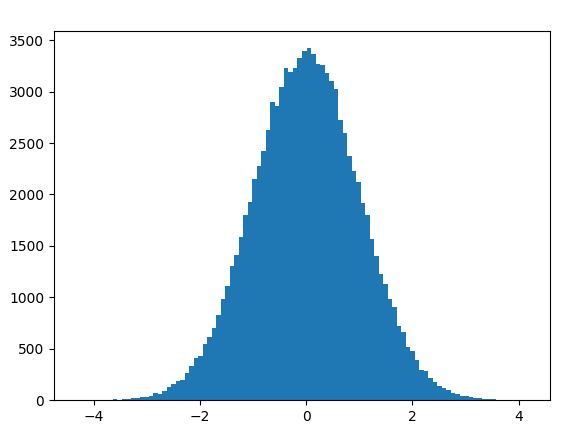
\includegraphics[width=0.7\textwidth]{figures/hist100BinsExample}
\end{figure}

\vspace*{-5mm}

\begin{itemize}
	\item identical data set as for $10$ bins
\end{itemize}

\end{frame}

%==============================================================

\begin{frame}[fragile]

\frametitle{Normalized histogram (area $1$), 100 bins}

\begin{figure}[ht]
	\centering
	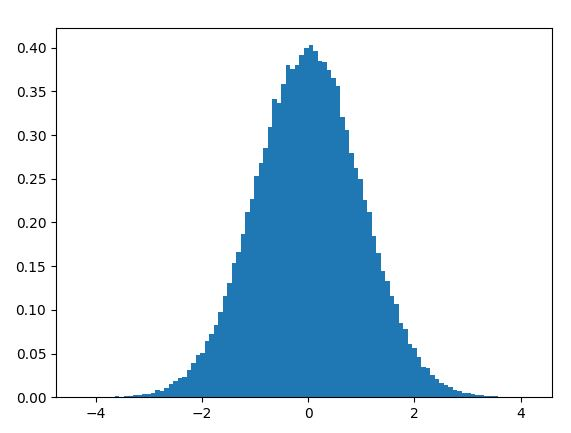
\includegraphics[width=0.7\textwidth]{figures/hist100BinsDensity}
\end{figure}

\vspace*{-5mm}

\begin{itemize}
	\item same histogram, except total area of rectangles is normalized to be $1$
\end{itemize}

\end{frame}

%==============================================================

\begin{frame}[fragile]

\frametitle{Normalized histogram with PDF}

\begin{figure}[ht]
	\centering
	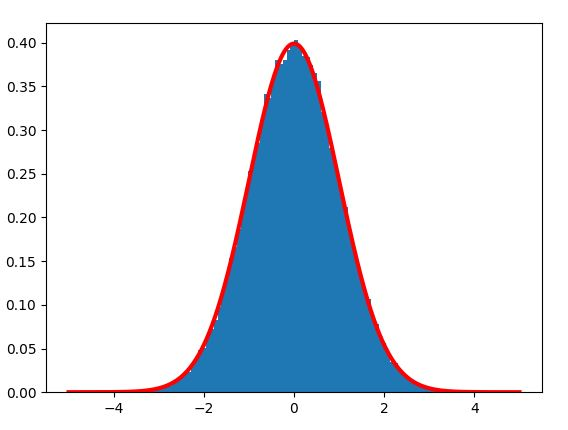
\includegraphics[width=0.7\textwidth]{figures/histWithpdf}
\end{figure}

\vspace*{-5mm}

\begin{itemize}
	\item[] red curve is \red{\emph{probability density function (PDF)}}
\end{itemize}

\end{frame}

%==============================================================

\begin{frame}[fragile]

\frametitle{Standard normal distribution}

Standard normal probability density function:
\[
\boxed{
f(x) = \frac{1}{\sqrt{2\pi}} e^{-x^2/2}}
\]

\begin{itemize}
	\item \emph{standard} normal distribution is a special case of distribution we'll see next week
	\item corresponds to parameters \red{$\mu = 0$} and \blue{$\sigma = 1$}
\end{itemize}

{\small
	\texttt{x = np.random.normal(\red{0.0}, \blue{1.0}, size=100000)}
}

\end{frame}

%==============================================================

\begin{frame}[fragile]

\frametitle{Probability density functions}

If $X$ is a random number drawn from a distribution with PDF $f(x)$, probability $X$ takes a value in interval $[a,b]$ is
\vspace*{-2mm}
\[
	\boxed{
\mathrm{P}(a \leq X \leq b) = \int_a^b f(x) dx}
\]
\vspace*{-5mm}
\begin{figure}[ht]
	\centering
	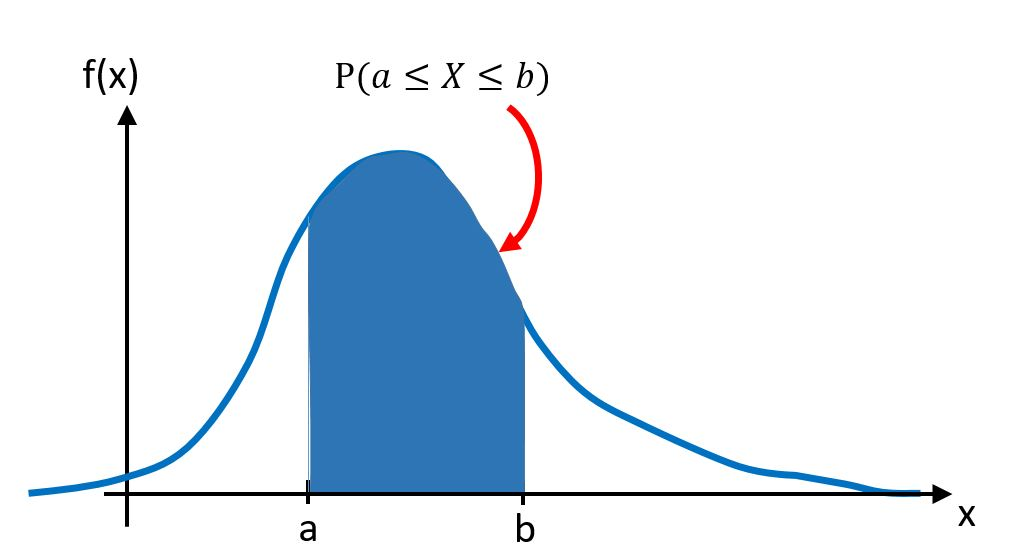
\includegraphics[width=.7\textwidth]{figures/genericPDF}
\end{figure}

\end{frame}

%==============================================================

\begin{frame}[fragile]

\frametitle{Properties of PDFs}

Two key properties of any probability density function:
\vspace*{5mm}
\begin{enumerate}
	\item \textbf{non-negativity} \\ \vspace*{2mm}
 $f(x) \geq 0$ for all $x$
 	\begin{itemize}
		\item since probability can't be negative
	\end{itemize}
	\item[]
	\item \textbf{normalization} \\ \vspace*{2mm}
	 entire area under $f(x)$ must be equal to $1$, since
	\[
\mathrm{P}(-\infty \leq X \leq \infty) = \int_{-\infty}^\infty f(x) dx = 1 
\] 
	\begin{itemize}
		\item reason for the $1/\sqrt{2\pi}$ factor in standard normal PDF
	\end{itemize}	
\end{enumerate}

\end{frame}

%==============================================================

\begin{frame}[fragile]

\frametitle{$2)$ Computing probabilities using standard \hspace*{8mm} normal distribution}

\begin{itemize}
	\item probability of random number $X$ drawn from standard normal distribution taking value in $[a,b]$:
	\[
	\mathrm{P}(a \leq X \leq b) = \frac{1}{\sqrt{2\pi}} \int_a^b  e^{-x^2/2} dx
	\]
	\item no exact expression exists for $\int_a^b e^{-x^2/2} dx$
	\begin{itemize}
		\item need to use numerical integration!
	\end{itemize}
	\item \textbf{Example:} use trapezoidal method to approximate $\mathrm{P}(1 \leq X \leq 2)$ when $X$ is drawn from standard normal distribution
\end{itemize}

\end{frame}

%==============================================================

\begin{frame}[fragile]

\frametitle{Example: fraction of standard normal numbers in $[1,2]$}

\vspace*{-2mm}
\begin{figure}[ht]
	\centering
	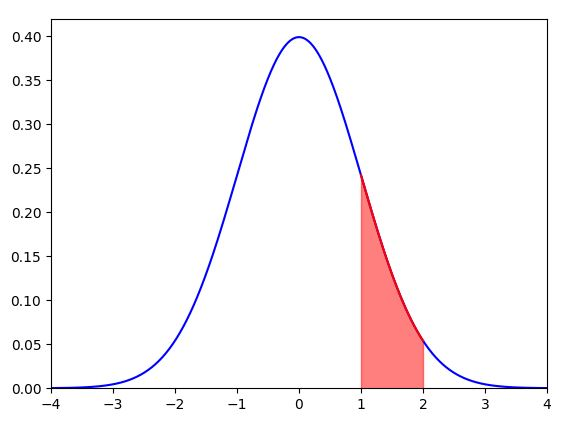
\includegraphics[width=.6\textwidth]{figures/stdnormal_12}
\end{figure}
\vspace*{-3mm}
\[
\mathsf{Red~shaded~area~} = \frac{1}{\sqrt{2\pi}} \int_1^2 e^{-x^2/2} dx \approx 0.1359
\]

\end{frame}

%==============================================================

\begin{frame}[fragile]

\frametitle{Python code: fraction of numbers in $[1,2]$}

\texttt{standardnormal.py}
\begin{lstlisting}[style=CStyle,basicstyle=\scriptsize]
# standardnormal
import numpy as np
import matplotlib.pyplot as plt

def f(x):
    return 1/(np.sqrt(2 * np.pi)) * np.exp(-x**2 / 2)

def trapezoidal(f, a, b, n):
    h = (b-a)/n
    f_sum = 0
    for i in range(1, n, 1):
        x = a + i*h
        f_sum = f_sum + f(x)
    return h*(0.5*f(a) + f_sum + 0.5*f(b))
\end{lstlisting}

\begin{itemize}
	\item lines 5--6: PDF of standard normal distribution
\end{itemize}

\end{frame}

%==============================================================

\begin{frame}[fragile]

\frametitle{Python code}

\texttt{standardnormal.py}---continued
\begin{lstlisting}[style=CStyle,basicstyle=\scriptsize]
a = 1
b = 2
prob_ab = trapezoidal(f, a, b, 100)
print('Probability X in range [{},{}] is: {:.4f}'.format(a, b, prob_ab))

x = np.linspace(-4, 4, 1000)
xab = np.linspace(a, b, 100)

plt.plot(x, f(x), 'b')             # standard normal pdf
plt.plot(xab,f(xab),'r')
plt.fill_between(xab,f(xab),color='r',alpha=0.5) #alpha=transparency
plt.axis([-4, 4, 0, 0.42])
plt.show()
\end{lstlisting}

\begin{itemize}
	\item line 3: approximate $\frac{1}{\sqrt{2\pi}} \int_1^2 e^{-x^2/2} dx$, $100$ panels
	\item line 7: $1 \leq x \leq 2$ for red shaded area plot
\end{itemize}

\end{frame}

%==============================================================

\begin{frame}[fragile]

\frametitle{Live demo: standard normal generation}

\begin{itemize}
	\item draw $N = 10^6$ random numbers from standard normal distribution
	\item[]
	\item for large $N$, expect fraction of random numbers $X$ in range $[1,2]$ to be close to
	\[
	\mathrm{P}(1 \leq X \leq 2)  = \frac{1}{\sqrt{2\pi}} \int_1^2 e^{-x^2/2} dx \approx \red{0.1359}
	\]
	\item[]
	\item live demo of \texttt{standardnormaldemo.py}
	\item[]
	\item observed fraction $\approx \red{0.136}$
	\item[]
\end{itemize}

\end{frame}

%==============================================================

\begin{frame}[fragile]

\frametitle{Python code}

\texttt{standardnormaldemo.py}
\begin{lstlisting}[style=CStyle,basicstyle=\scriptsize]
# standardnormaldemo
import numpy as np

N = 1000000
x = np.random.normal(0.0, 1.0, size=N)
a = 1
b = 2
num_ab = 0
for k in range(0, len(x)):
    if a <= x[k] <= b:
        num_ab += 1

print('{} standard normal random numbers'.format(N))
print('Fraction of random numbers in range [{},{}] = {:.4f}'.format(a, b, num_ab/N))
\end{lstlisting}

\begin{itemize}
	\item lines 8--12: \texttt{for} loop counts number of random numbers $x$ satisfying $1 \leq x \leq 2$
\end{itemize}

\end{frame}

%==============================================================

\begin{frame}[fragile]

\frametitle{Lecture summary}

\begin{enumerate}
	\item standard normal distribution
	\begin{itemize}
		\item drawing \texttt{N} random samples using \texttt{numpy.random.normal(0.0, 1.0, size=N)}
	\end{itemize}
	
	\item[]
	
	\item compute probability $\mathrm{P}(a \leq X \leq b)$ for standard normal distribution
	\begin{itemize}
		\item needs numerical integration using PDF
		\[
			f(x) = \frac{1}{\sqrt{2\pi}} \int_a^b e^{-x^2/2} dx
		\]
	\end{itemize}
	
\end{enumerate}

\end{frame}

\end{document}